%% ----------------------------------------------------------------
%% SETTINGS
%% ----------------------------------------------------------------
\documentclass[../et.tex]{subfiles}

%% ----------------------------------------------------------------
%% BEGIN
%% ----------------------------------------------------------------
\begin{document}

%% ----------------------------------------------------------------
%% DOCUMENT
%% ----------------------------------------------------------------
Se utilizará un microcontrolador SAM4S8B, debido a la necesidad de realizar funciones complejos y para cumplir ambos requerimientos funcionales. Es así que se implementará en el mismo:

\begin{itemize}
  \item Control digital de la corriente generada a lazo cerrado
  \item Control de generación de corriente a través de PWM
  \item Interfaz con la PC a través de USB
  \item Generación de clock para el ADC externo a través de PWM
  \item Control de ADC externo utilizando SPI
  \item Muestreo utilizando ADC interno (opcional)
  \item Procesamiento de datos adquiridos
  \item Guardado de información de calibración en EEPROM externa
\end{itemize}

Por su complejidad, se describirá el esquemático de acuerdo a sus distintes partes funcionales.

%% ----------------------------------------------------------------
\subsubsection{Fuente de alimentación}
%% ----------------------------------------------------------------
Para poder alimentar al microcontrolador, se utilizó la fuente de \SI{3.3}{V}. De esta manera, se procedió a conectar varios capacitores de desacople, tanto de \SI{10}{\micro F} como de \SI{0.1}{\micro F}, de manera de filtrar los diferentes rangos de frecuencia que estos permiten. En la \autoref{fig:arm-supply} se puede observar los componentes utilizados.

\begin{figure}[!htbp]
  \centering
  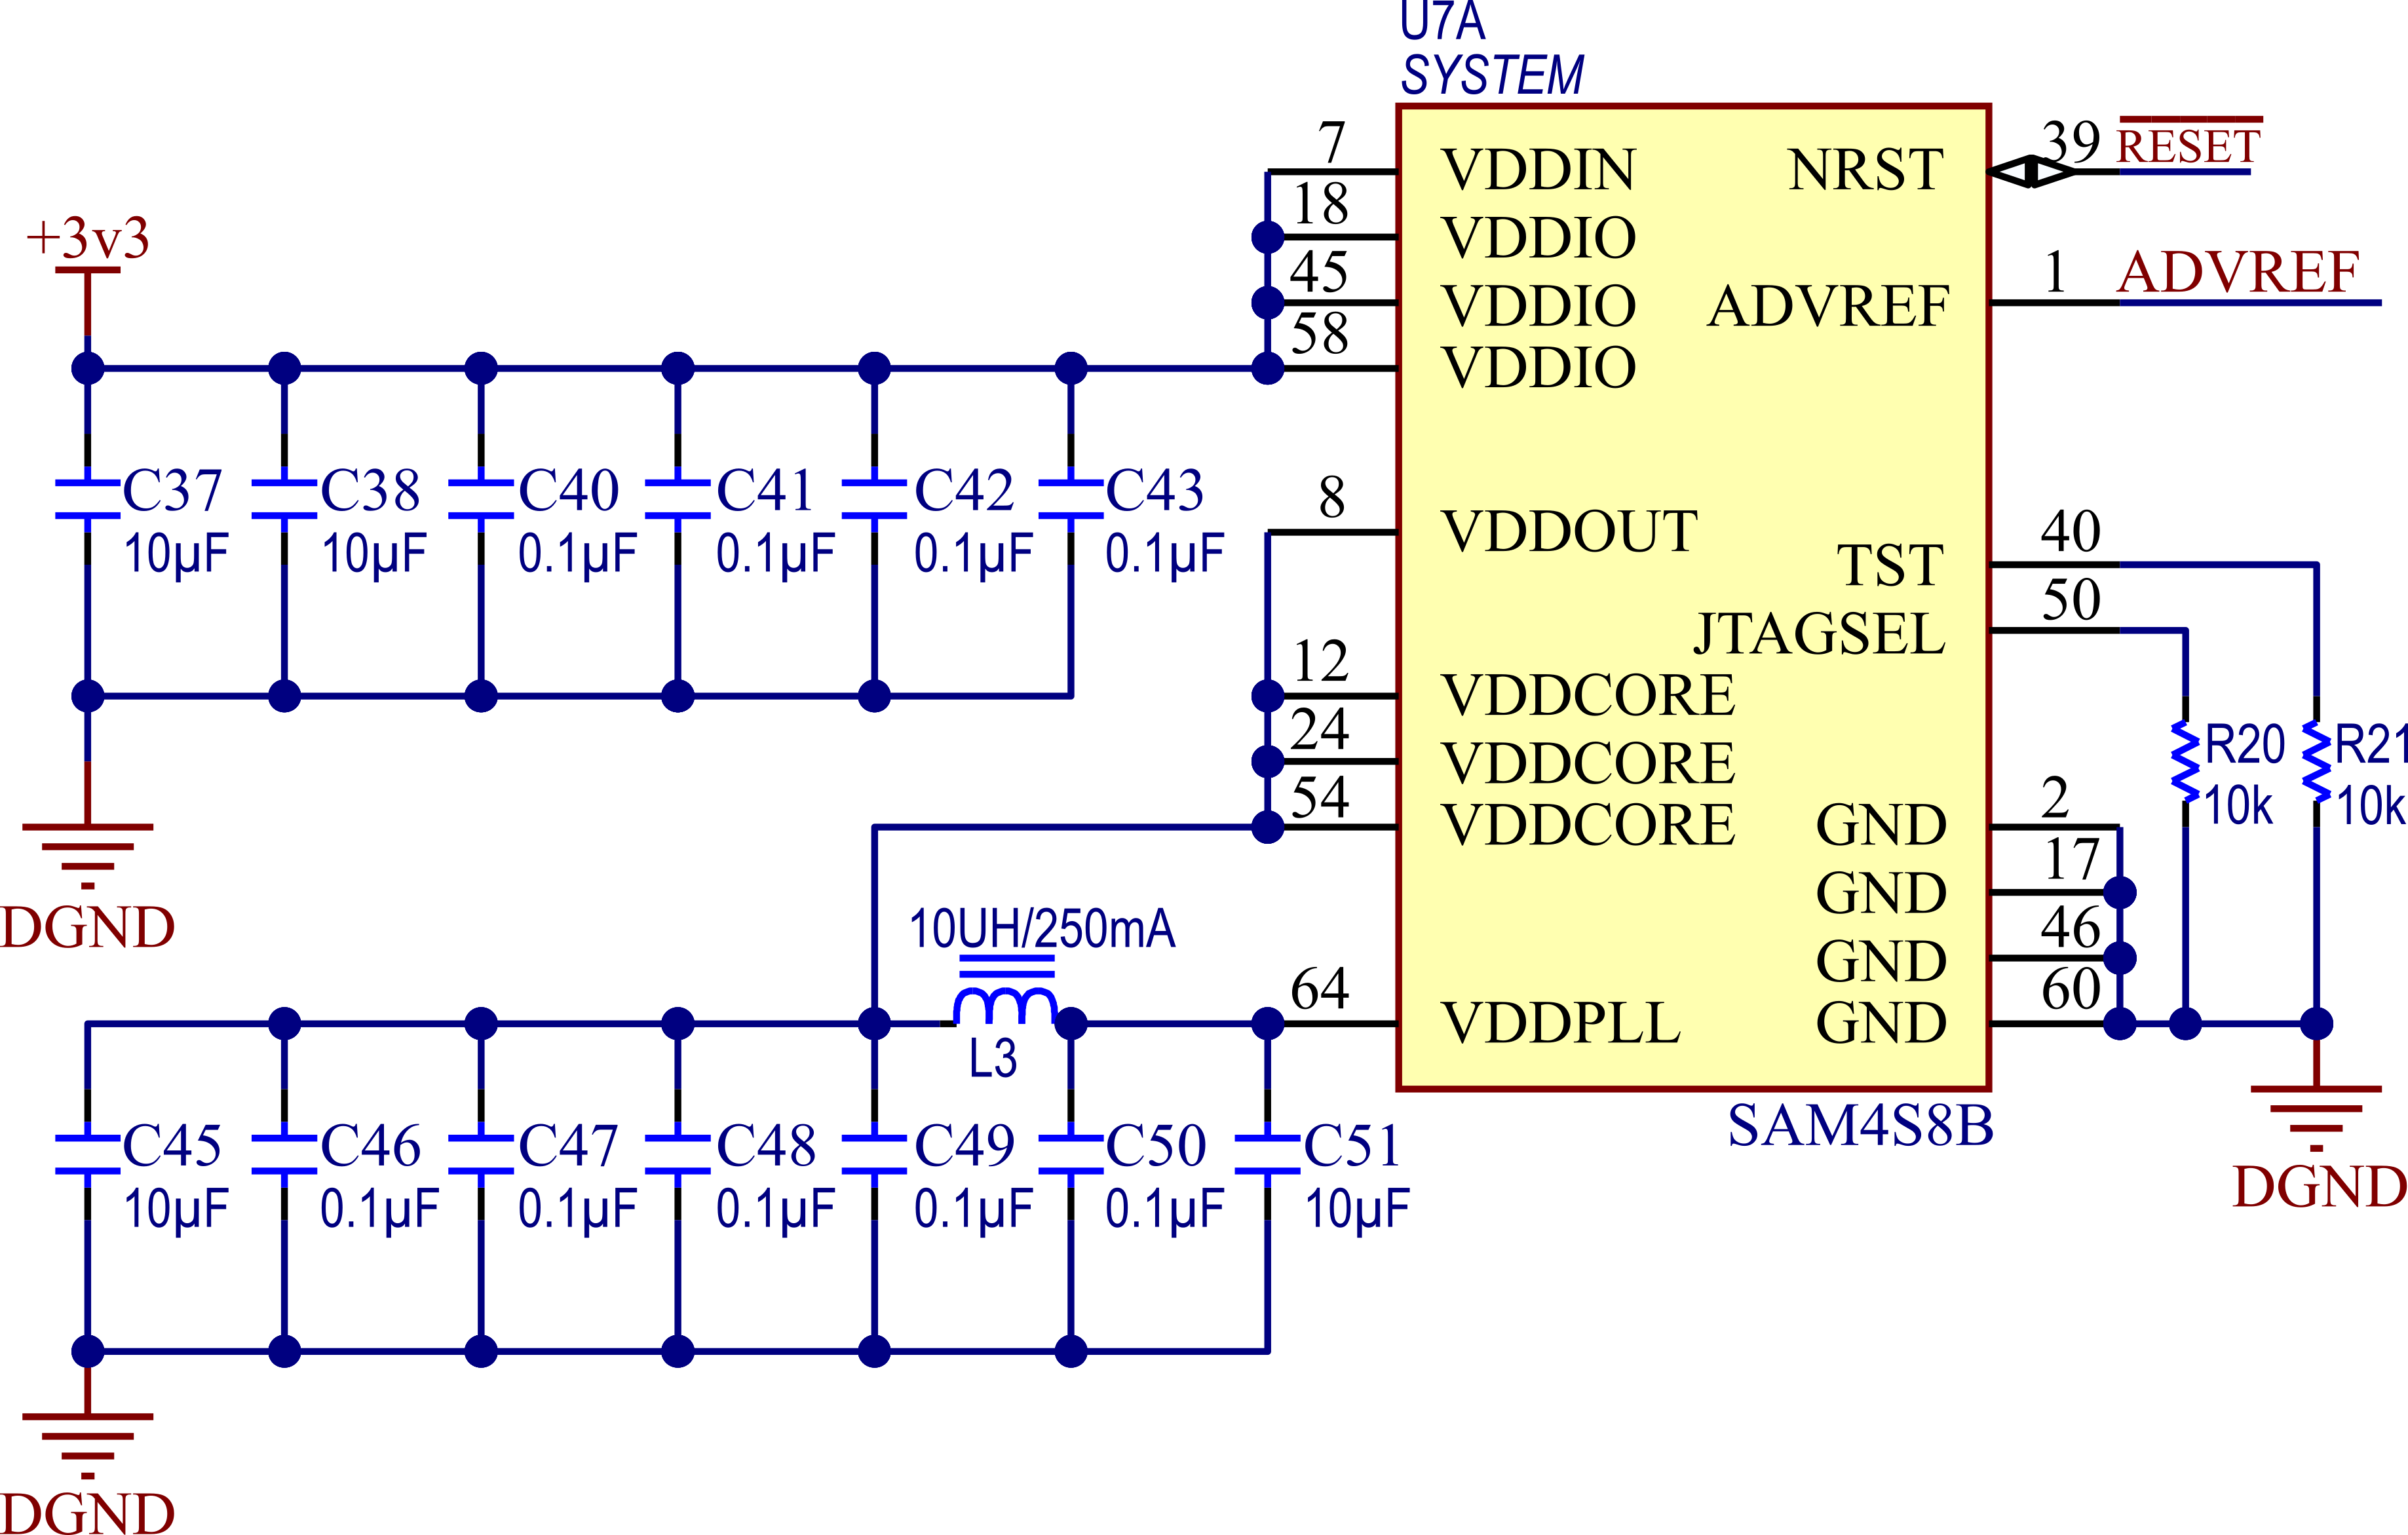
\includegraphics[scale=1.5]{../images/arm-supply.png}
  \caption{Alimentación del microcontrolador}
  \label{fig:arm-supply}
\end{figure}

%% ----------------------------------------------------------------
\subsubsection{Fuente de alimentación de referencia del ADC interno}
%% ----------------------------------------------------------------
Se agregó una fuente de referencia para el ADC.Se eligió el integrado ISL21010\_3V0, por su facilidad de uso y disponibilidad. En la \autoref{fig:arm-fuente-ref} se puede observar el esquemático utilizado.

\begin{figure}[!htbp]
  \centering
  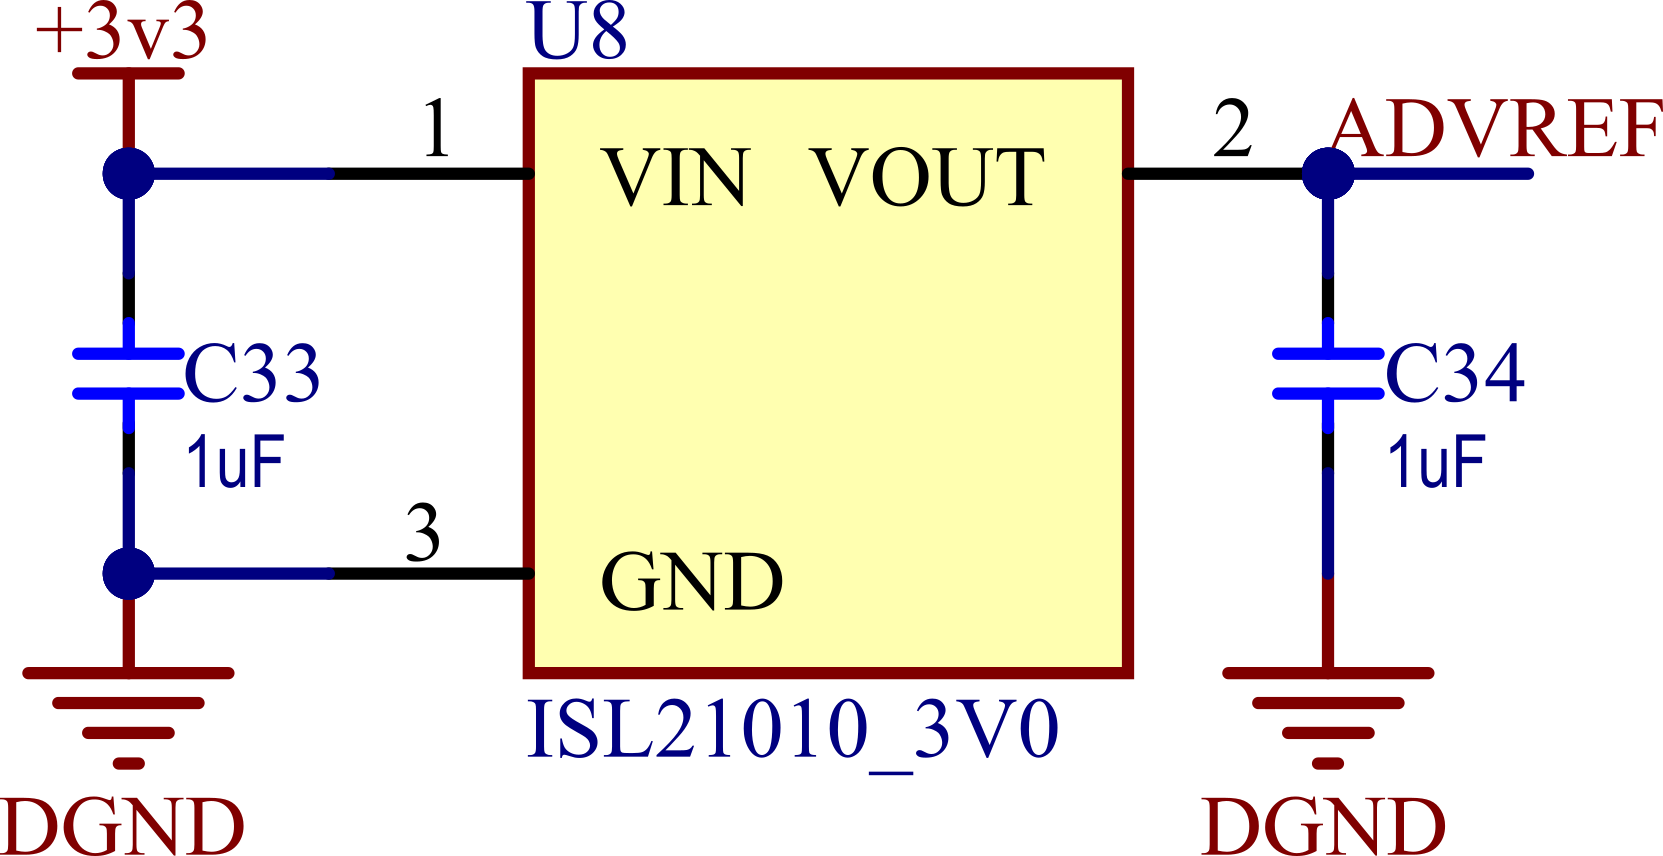
\includegraphics[scale=1.5]{../images/arm-fuente-ref.png}
  \caption{Fuente de referencia del ADC del microcontrolador}
  \label{fig:arm-fuente-ref}
\end{figure}

%% ----------------------------------------------------------------
\subsubsection{Puertos de entrada y salida}
%% ----------------------------------------------------------------
En estos pines de entrada y salida es donde está concentradas la mayoría de las funciones que se irán explicando por cada grupo. Las conexiones de ambos puertos se pueden ver en la \autoref{fig:arm-gpio-port-a} y en la \autoref{fig:arm-gpio-port-b}.


\begin{figure}[!htbp]
  \centering
  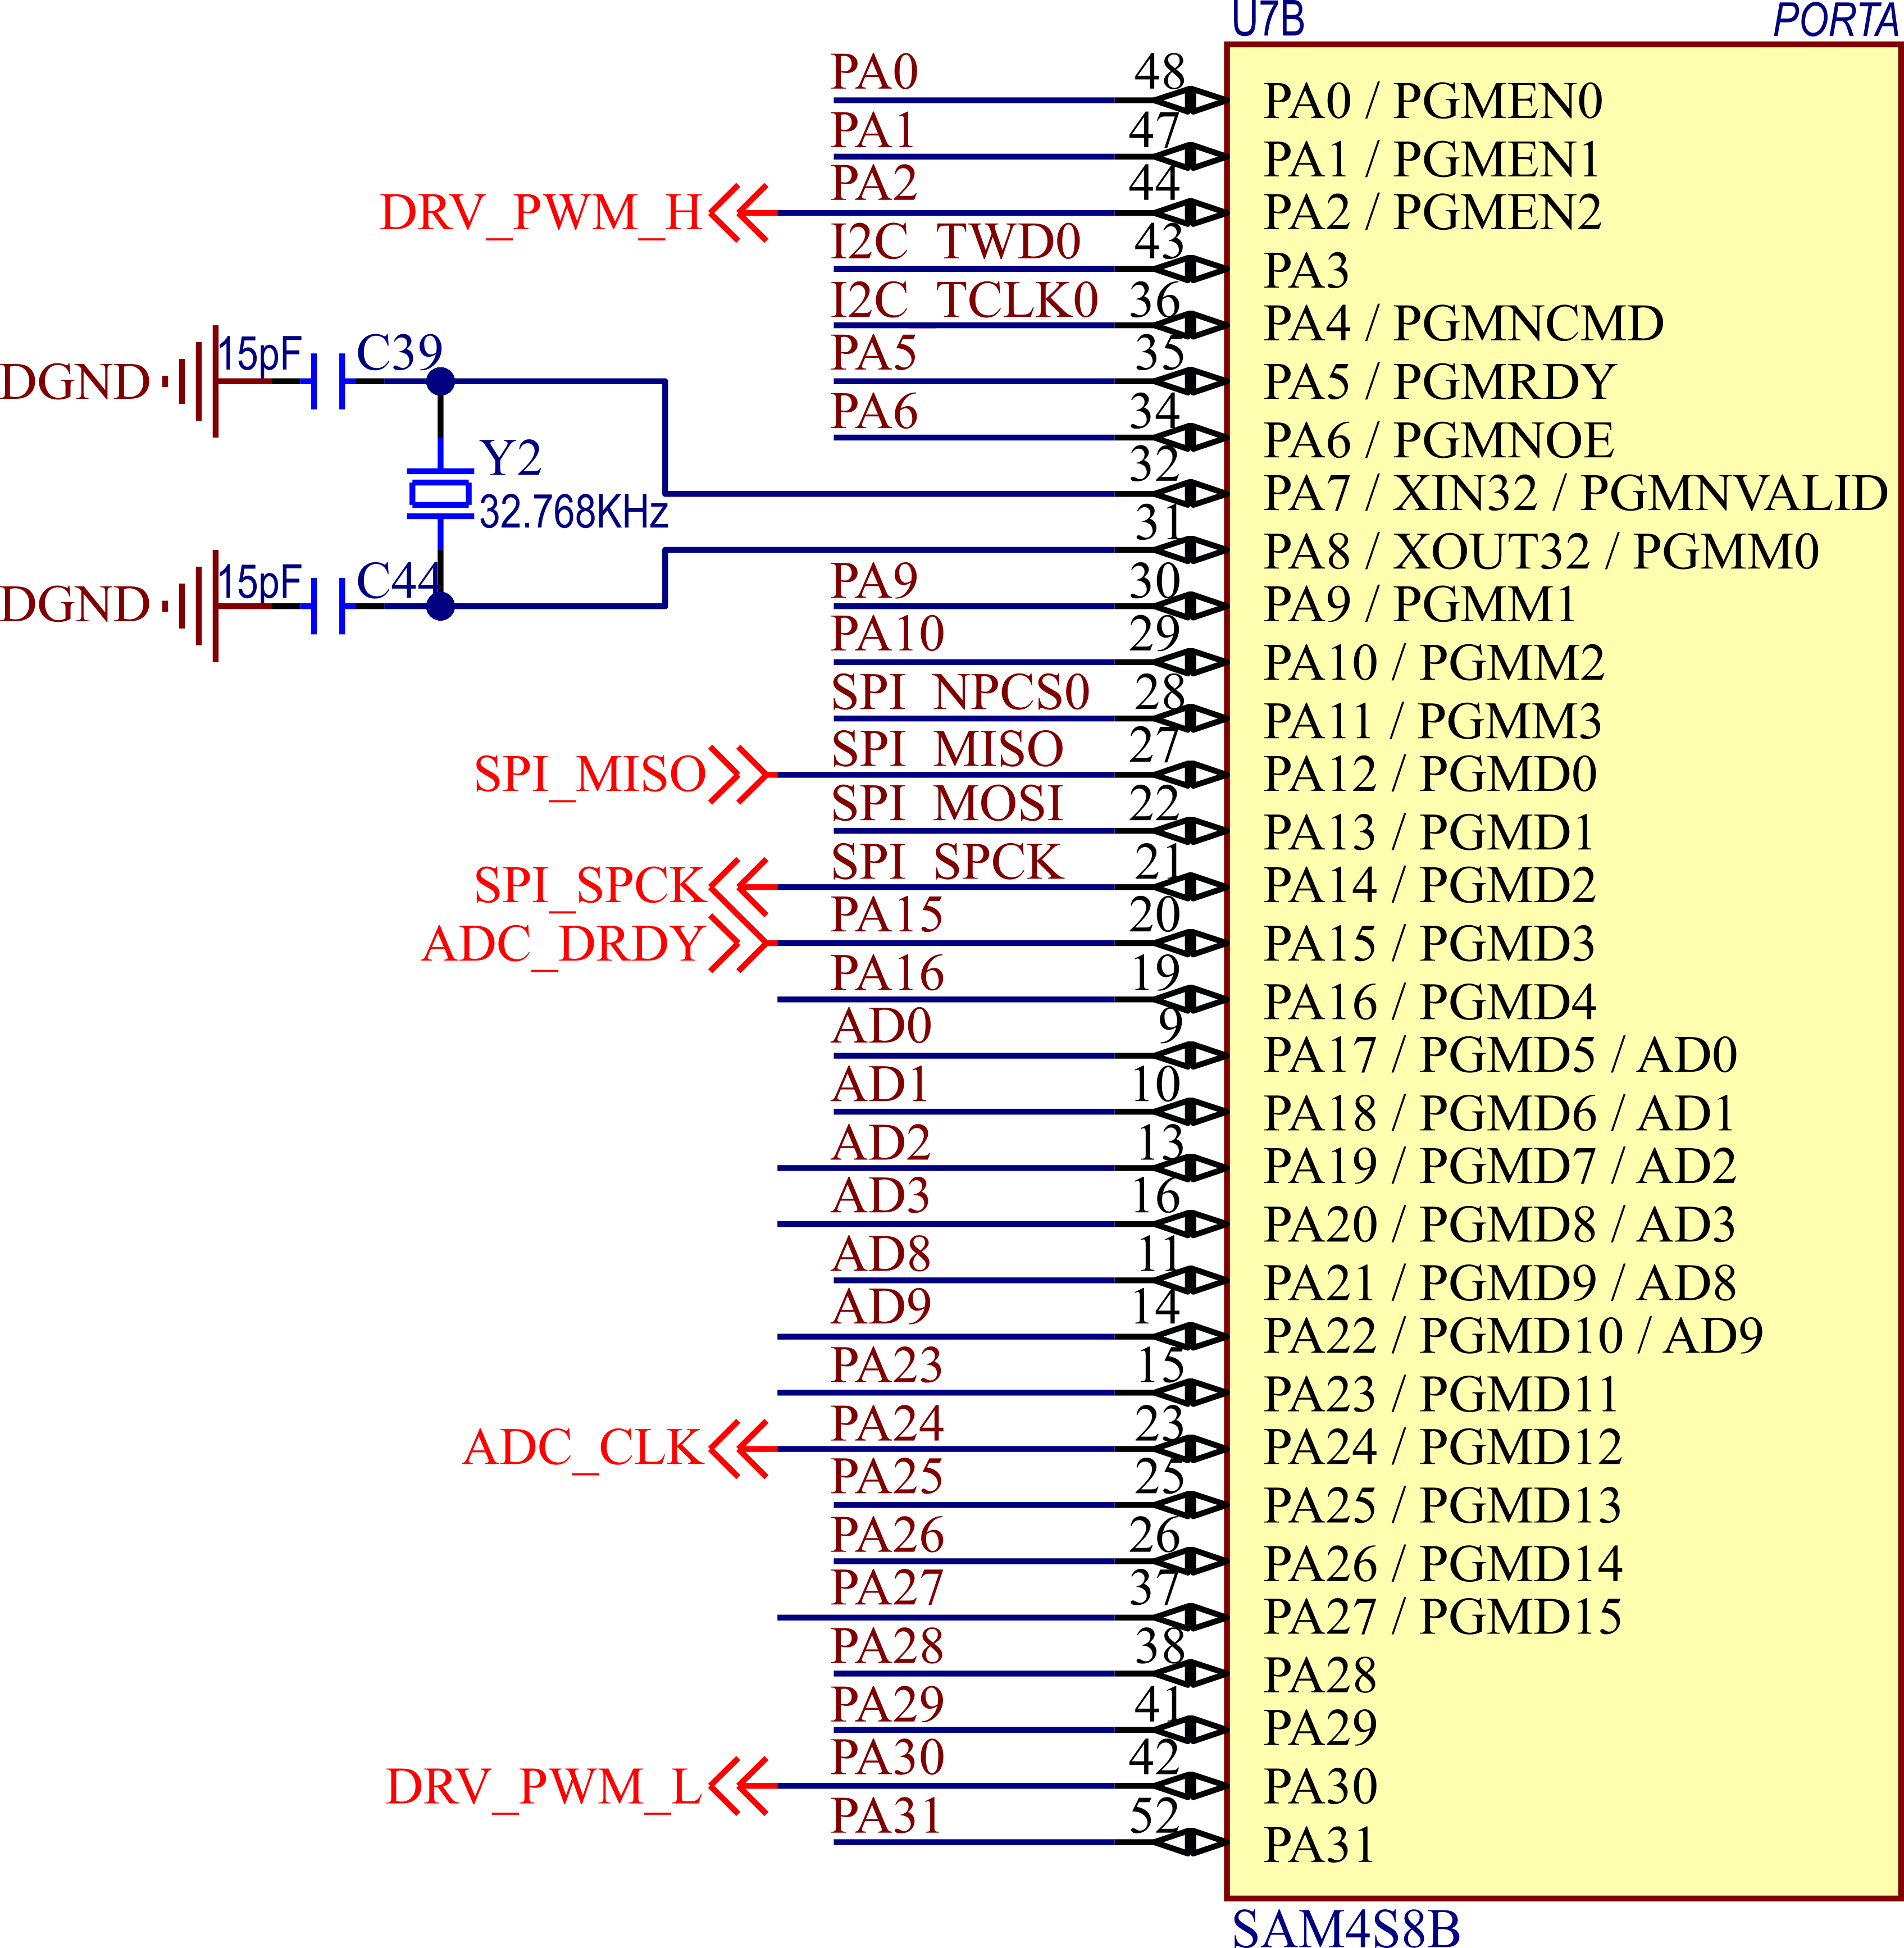
\includegraphics[scale=1.5]{../images/arm-gpio-port-a.png}
  \caption{Pines del puerto A del microcontrolador}
  \label{fig:arm-gpio-port-a}
\end{figure}

\begin{figure}[!htbp]
  \centering
  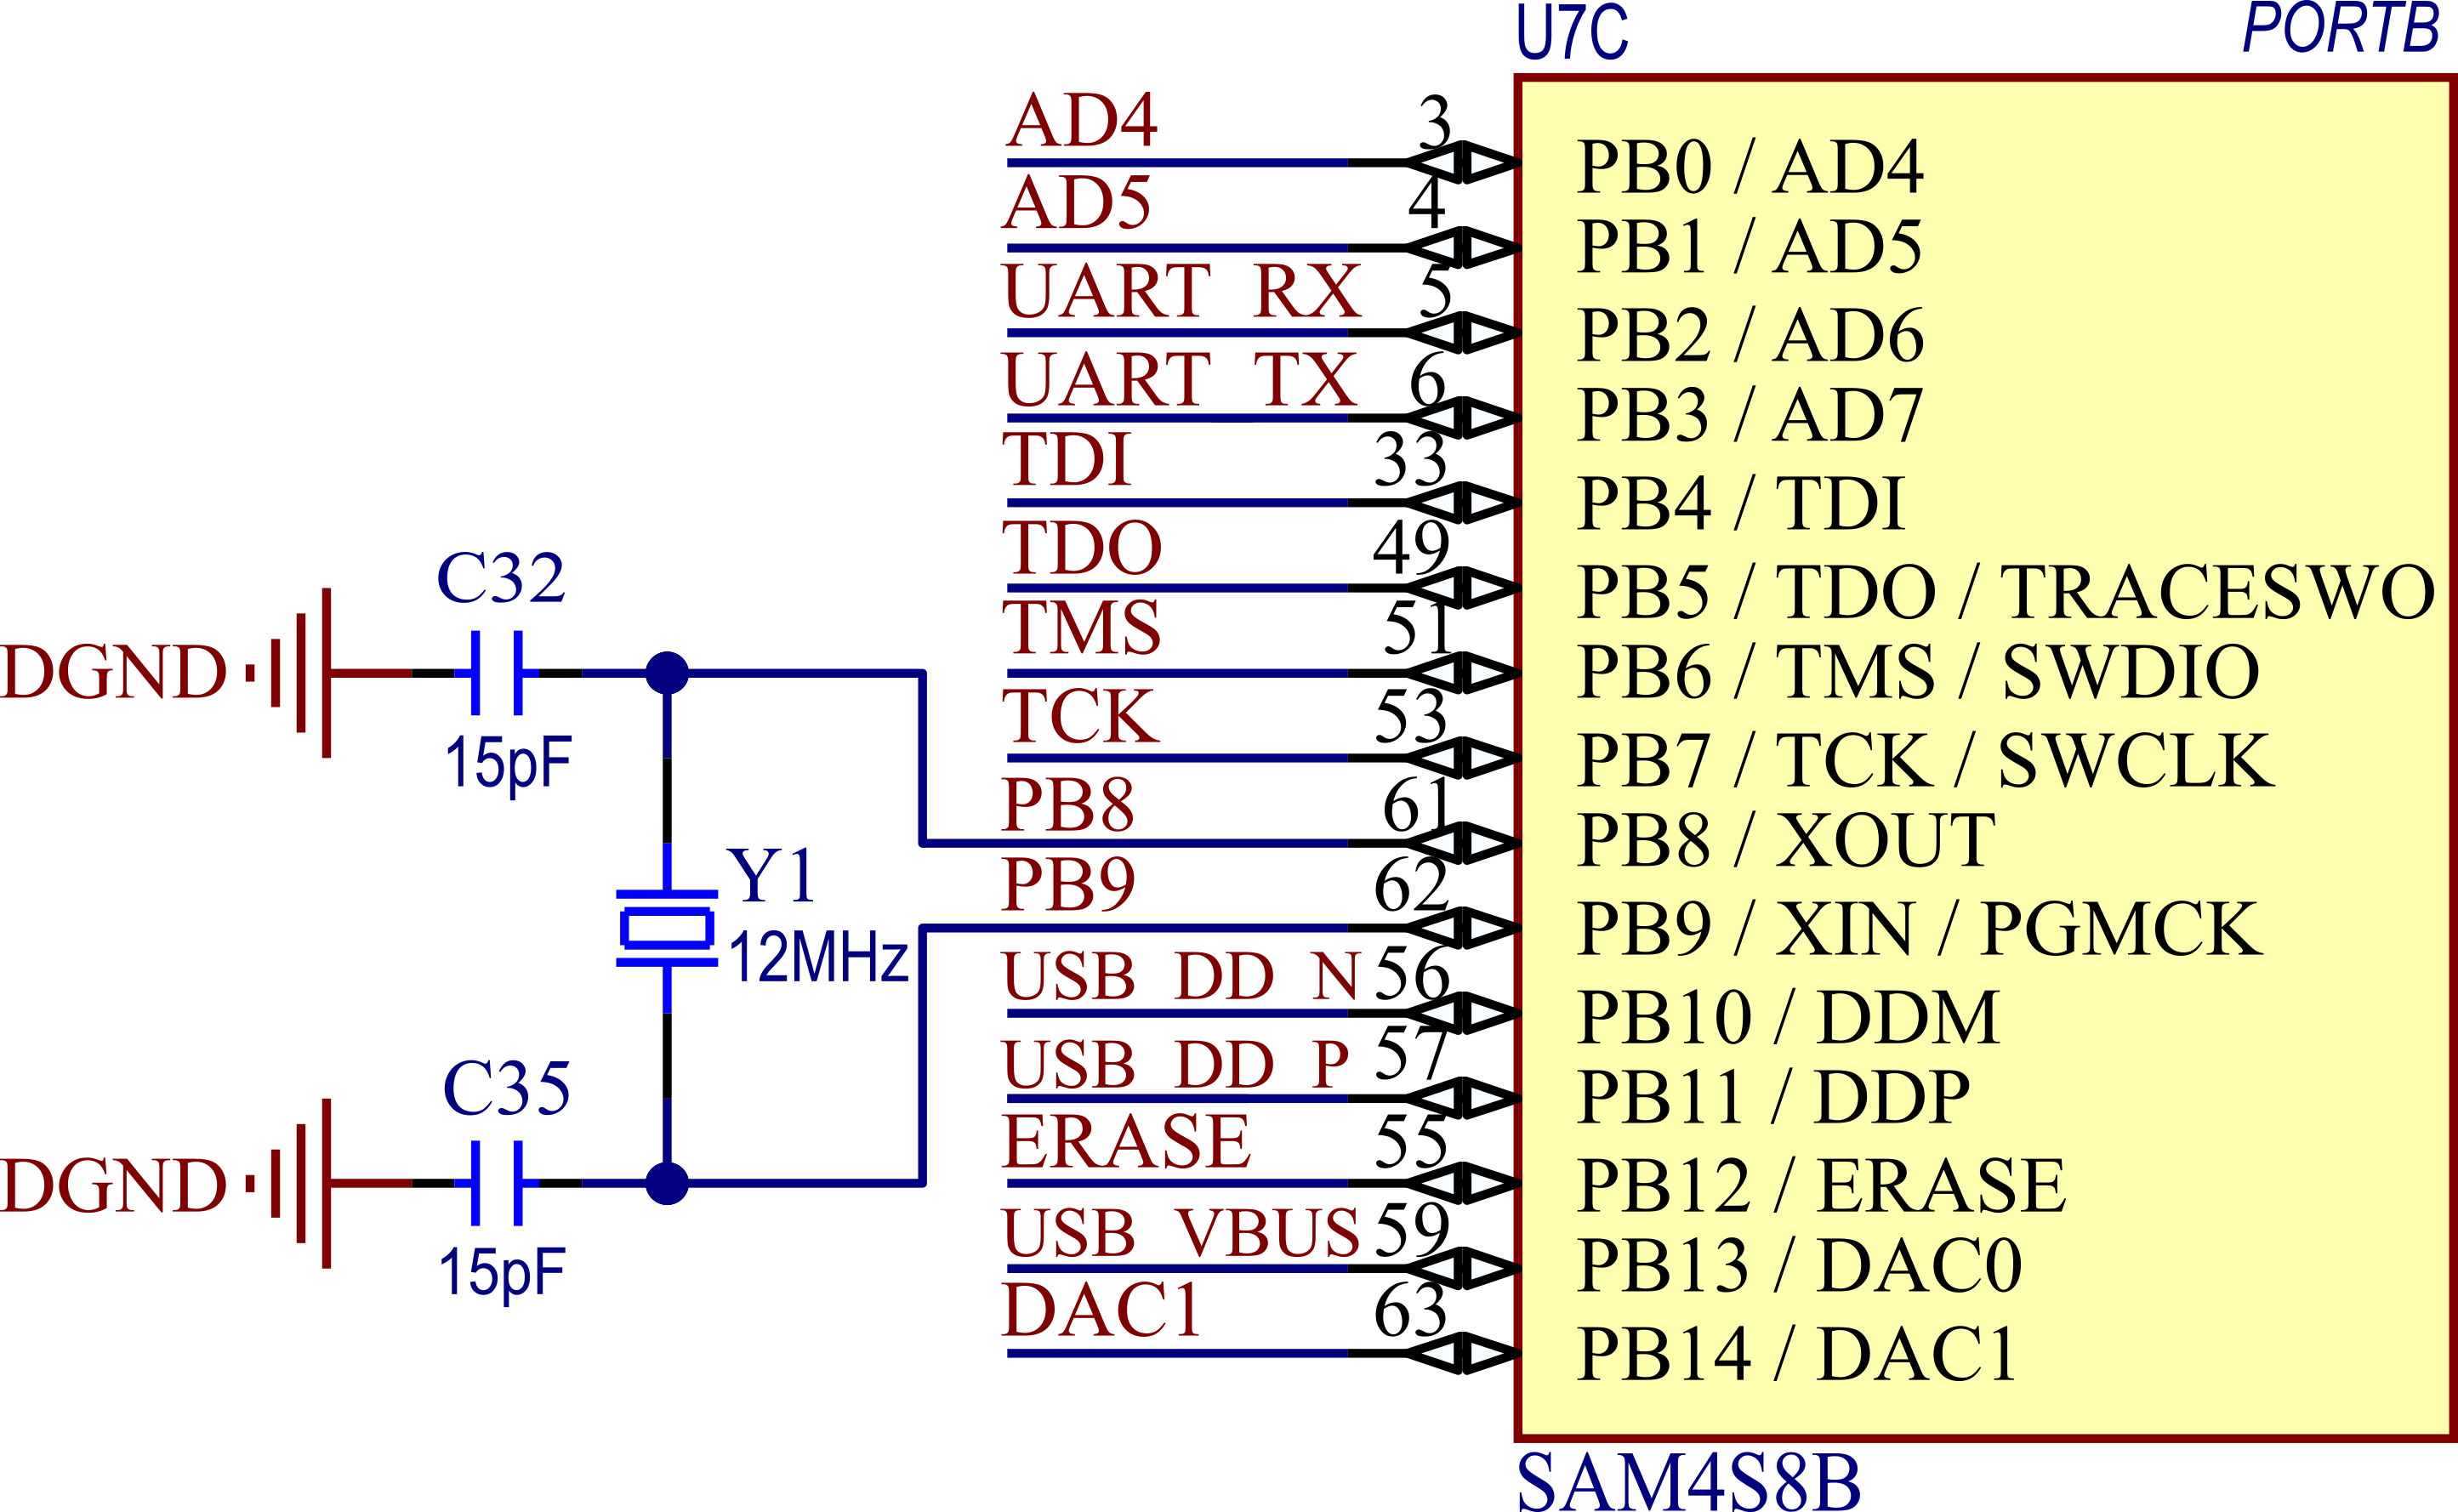
\includegraphics[scale=1.5]{../images/arm-gpio-port-b.png}
  \caption{Pines del puerto B del microcontrolador}
  \label{fig:arm-gpio-port-b}
\end{figure}

Se han conectado también dos cristales que servirán para control del puerto USB ($Y1$) y para la función RTC del microcontrolador ($Y2$).

Cabe destacar algunas señales que se verán en otras etapas, tales como:

\begin{itemize}
  \item DRV\_PWM\_H, DRV\_PWM\_L: se conectan a la entrada diferencial de control del driver del MOSFET.
  \item SPI\_MISO, SPI\_SPCK: sirven para comunicación entre el ADC y el microcontrolador.
  \item ADC\_CLK: clock del ADC
\end{itemize}

%% ----------------------------------------------------------------
\subsubsection{Conexión JTAG/SWD}
%% ----------------------------------------------------------------
Se agregaron también las conexiones necesarias para colocar un header JTAG/SWD de manera de poder programar el microcontrolador. Como se puede observar en la \autoref{fig:arm-jtag}, se agregaron también resistencias pull-up de \SI{100}{k\ohm} y un capacitor de desacople en la salida de \SI{3.3}{V}.

\begin{figure}[!htbp]
  \centering
  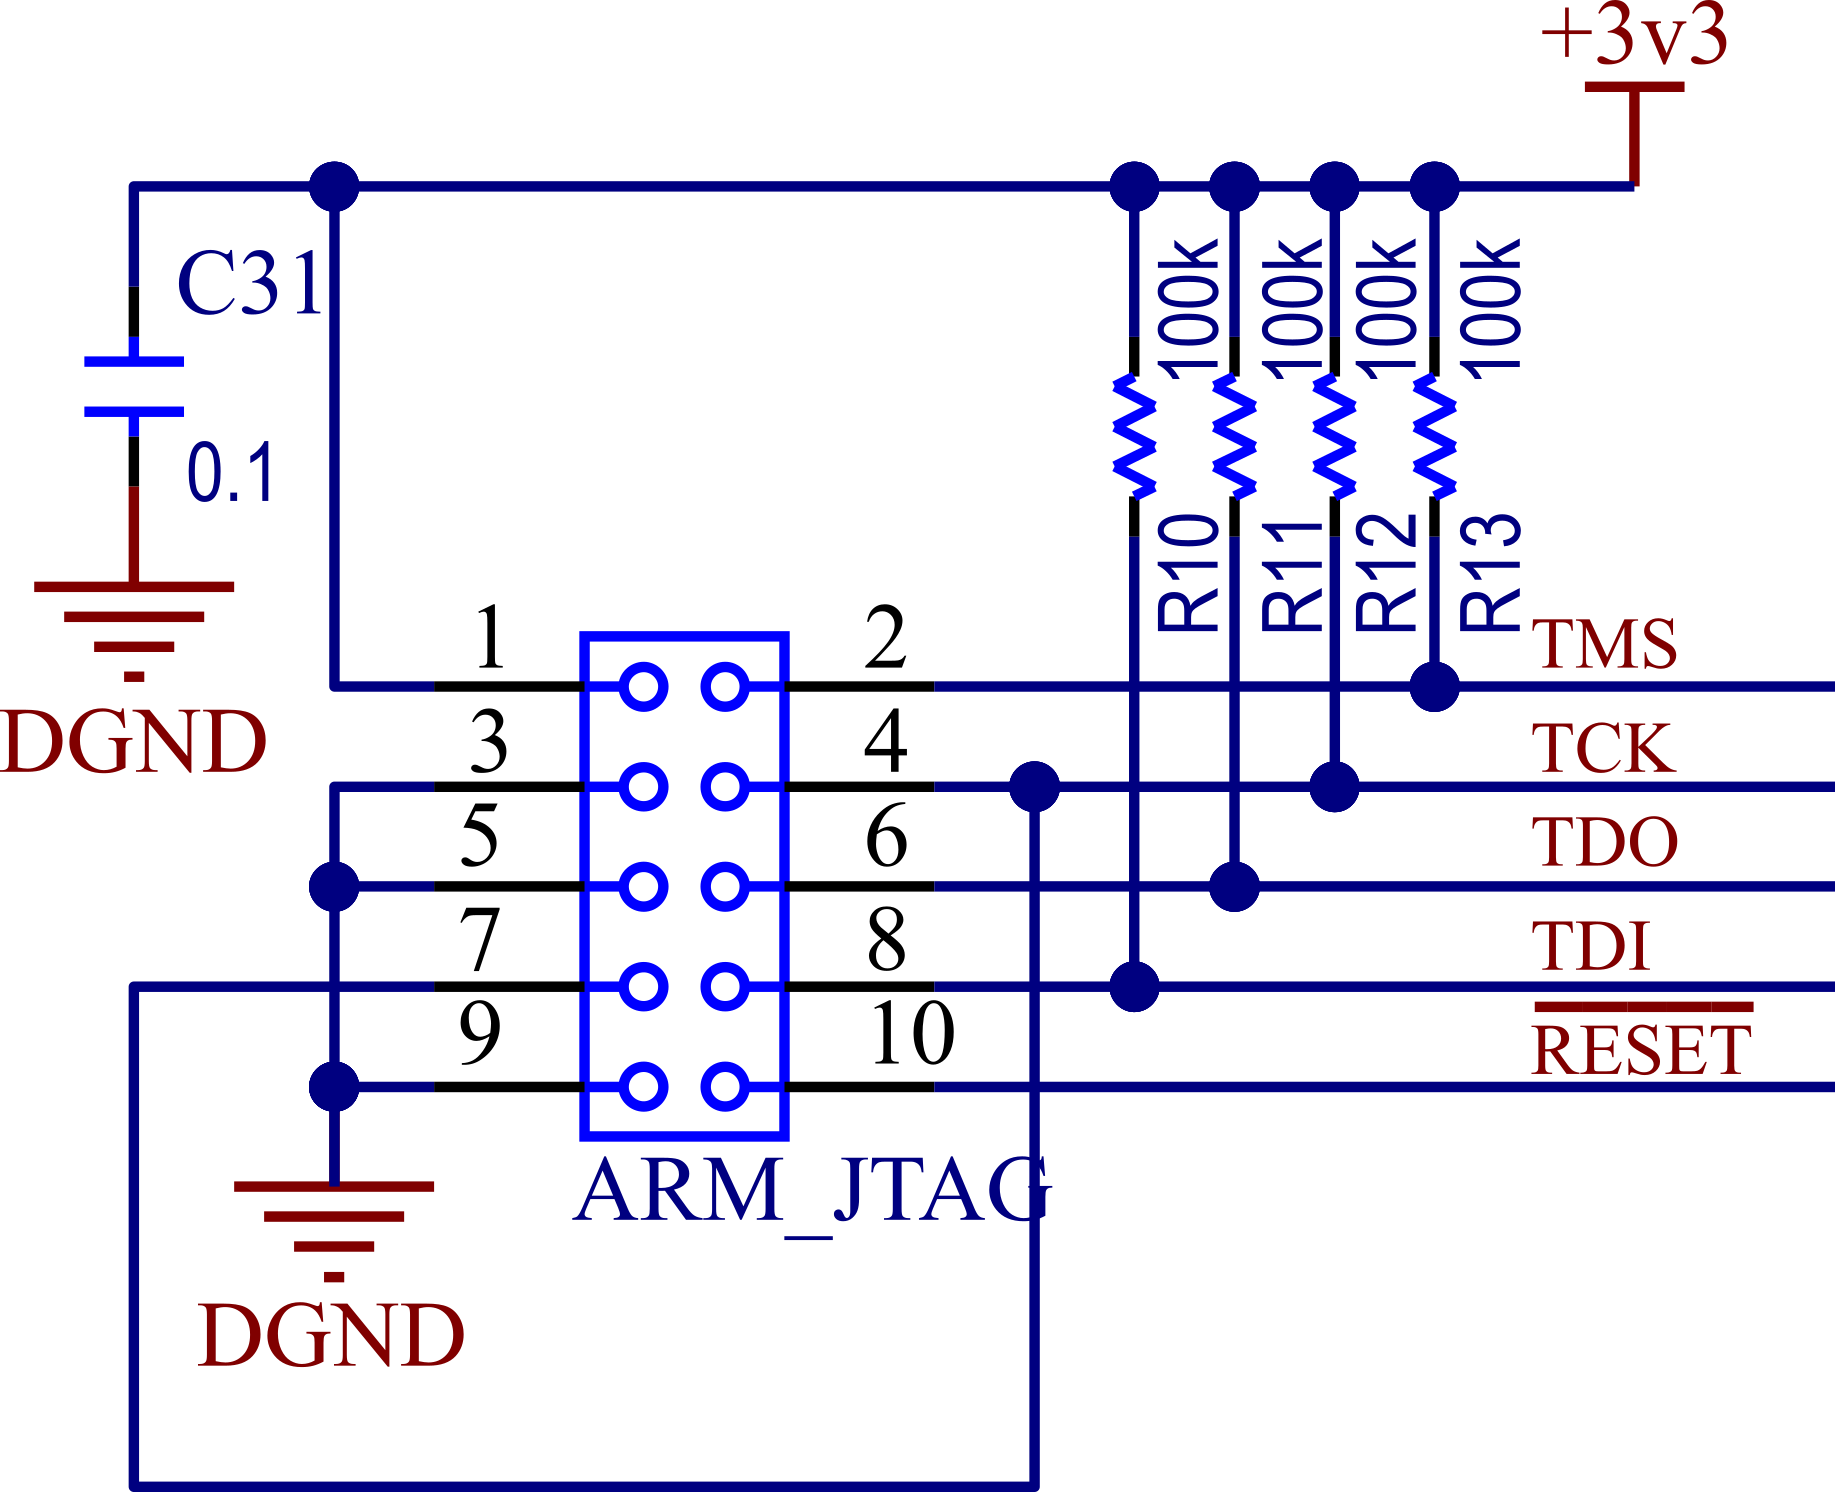
\includegraphics[scale=1.5]{../images/arm-jtag.png}
  \caption{Conexión JTAG/SWD del microcontrolador}
  \label{fig:arm-jtag}
\end{figure}

%% ----------------------------------------------------------------
\subsubsection{Conexión USB}
%% ----------------------------------------------------------------
La conexión USB consta de 2 señales:

\begin{itemize}
  \item USB\_VBUS: genera la interrupción en el microcontrolador cuando el puerto USB es conectado a la PC, teniendo que adecuarse la tensión de \SI{5}{V} de entrada con un divisor resistivo.
  \item USB\_DD: señal diferencial de transmisión de datos, terminada cada una con una resistencia de \SI{22}{\ohm} de manera de mejorar la adaptación de impedancias.
\end{itemize}

Se utilizó en este caso un puerto mini-USB, siendo uno de los más usados y comunes en la industria. En la \autoref{fig:arm-usb} se puede observar el esquemático.

\begin{figure}[!htbp]
  \centering
  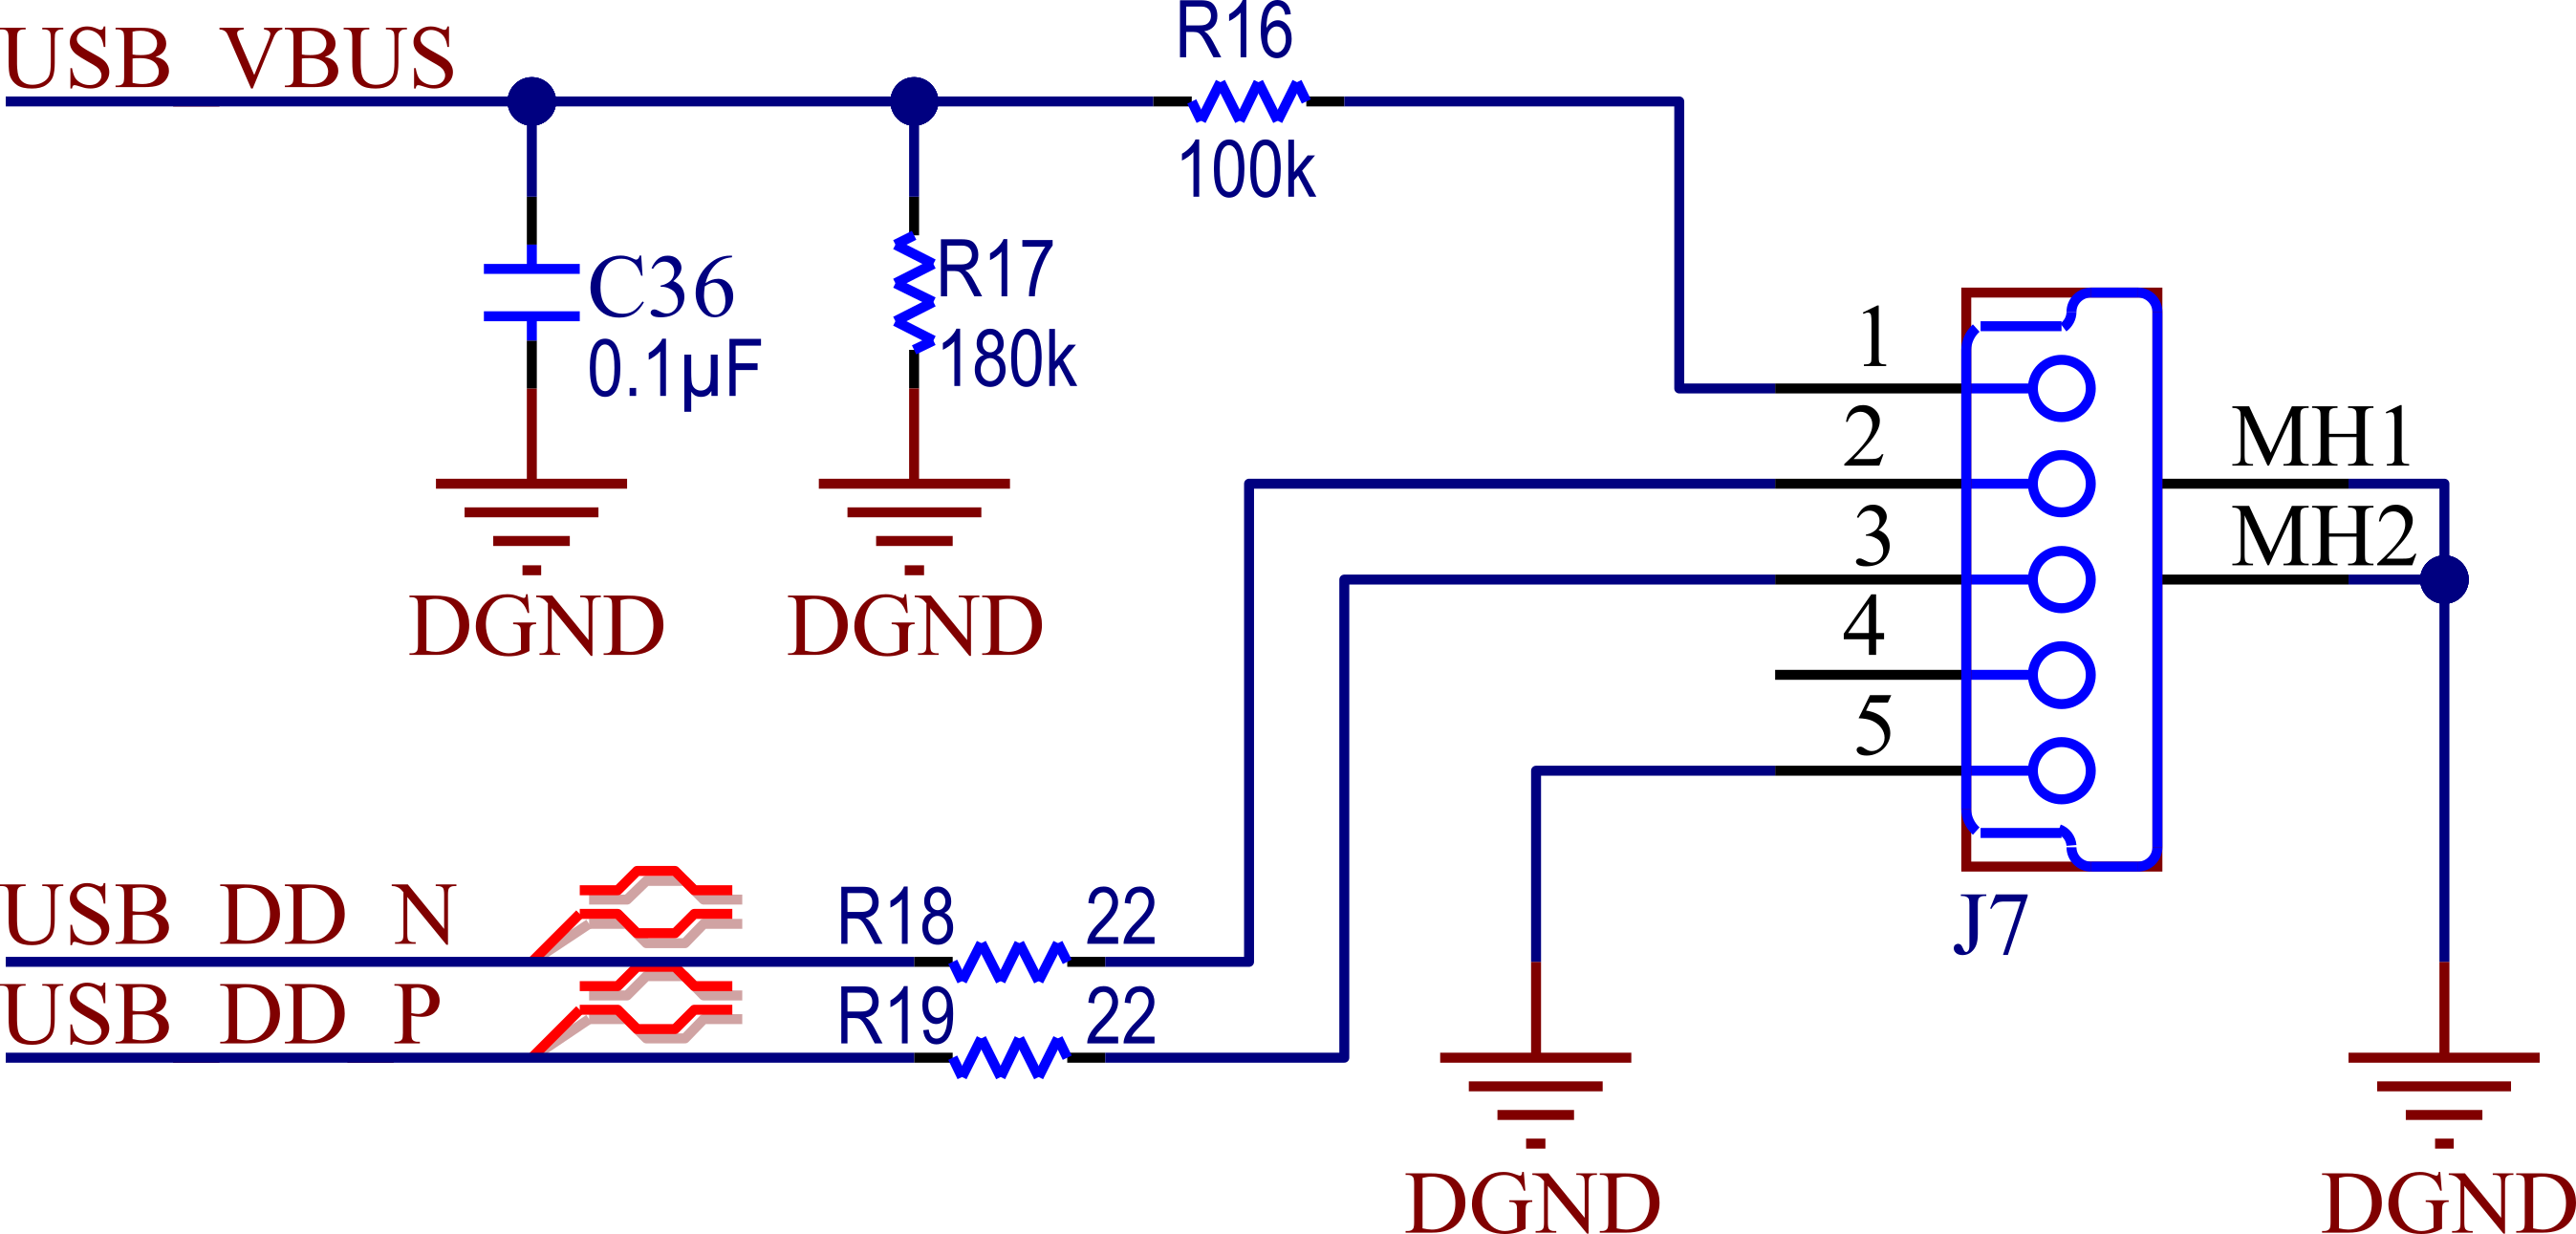
\includegraphics[scale=1.5]{../images/arm-usb.png}
  \caption{Conexión USB del microcontrolador}
  \label{fig:arm-usb}
\end{figure}

%% ----------------------------------------------------------------
\subsubsection{EEPROM}
%% ----------------------------------------------------------------
Se ha optado por utilizar una memoria EEPROM para guardar los datos de calibración del instrumento. Se conecta mediante I$^2$C.

En la \autoref{fig:arm-eeprom} se puede observar los componentes utilizados. Se agregaron dos resistencias pull-up y un capacitor de desacople.

\begin{figure}[!htbp]
  \centering
  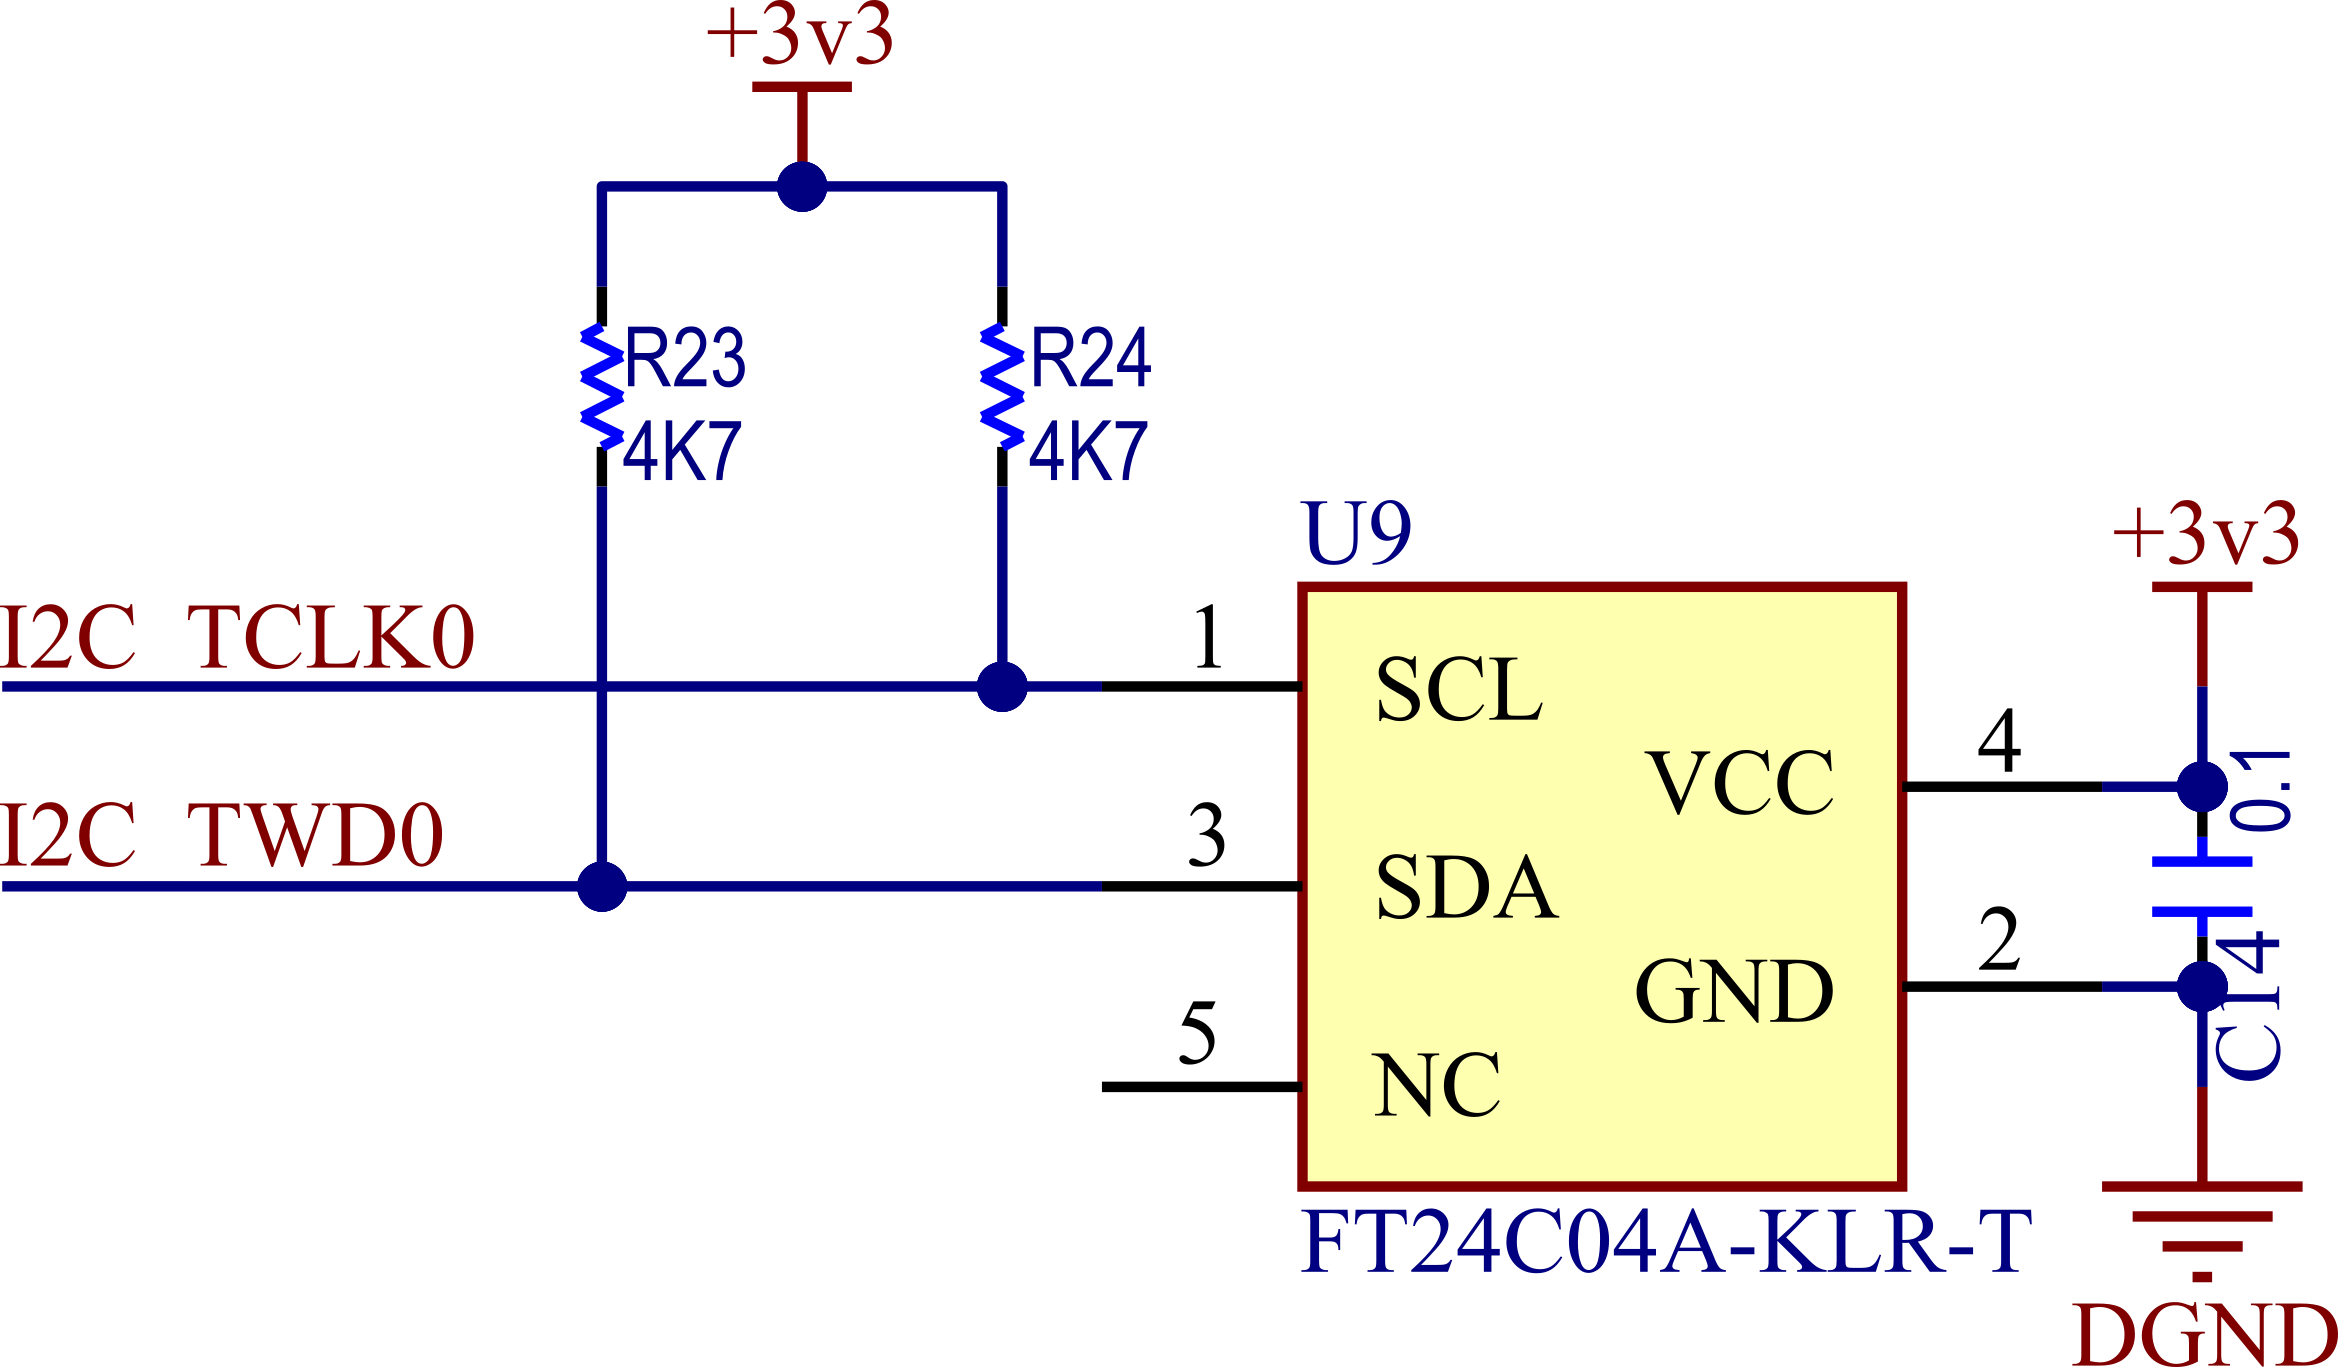
\includegraphics[scale=1.5]{../images/arm-eeprom.png}
  \caption{Conexión EEPROM al microcontrolador}
  \label{fig:arm-eeprom}
\end{figure}

%% ----------------------------------------------------------------
\subsubsection{RESET y ERASE}
%% ----------------------------------------------------------------
Se dejaron dos header expuestos, con el objetivo de tener fácil acceso en caso de graves problemas en el microcontrolador. Estas conexiones son las de RESET y ERASE, permitiendo reiniciar y borrar la memoria, respectivamente. En ambos casos no fue necesario agregar una resistencia de pull-up o pull-down, ya que el microcontrolador las trae integradas dentro del mismo.

En la \autoref{fig:arm-reset-erase} se pueden observar ambos header.

\begin{figure}[!htbp]
  \centering
  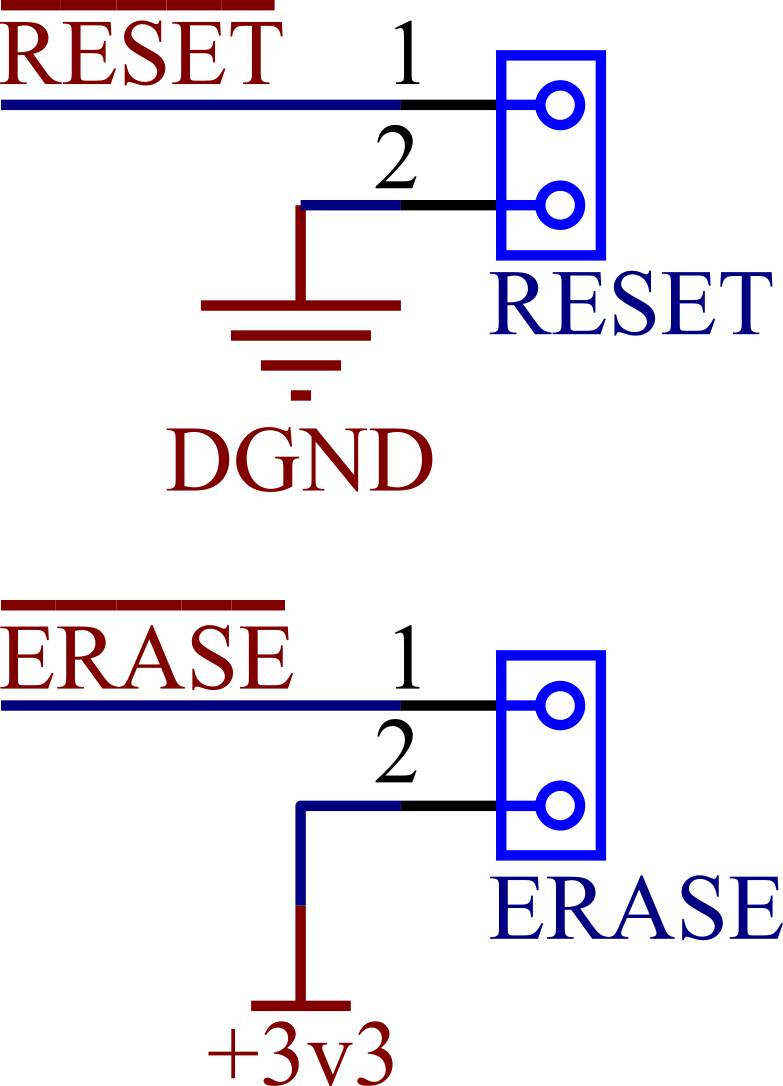
\includegraphics[scale=1.5]{../images/arm-reset-erase.png}
  \caption{Header RESET y ERASE del microcontrolador}
  \label{fig:arm-reset-erase}
\end{figure}

%% ----------------------------------------------------------------
\subsubsection{Otras conexiones}
%% ----------------------------------------------------------------
Además de las ya nombradas, se dejaron ciertos pines expuestos para tener mayor flexibilidad ante futuros cambios:

\begin{itemize}
  \item Header que deja expuesto el DAC, ADC, UART y demás pines generales de entrada y salida, como se puede ver en la \autoref{fig:arm-header}.
  \item Botón, se puede ver en la \autoref{fig:arm-button}.
  \item LEDs, se puede ver en la \autoref{fig:arm-leds}.
\end{itemize}

\begin{figure}[!htbp]
  \begin{subfigure}[b]{\textwidth}
    \centering
    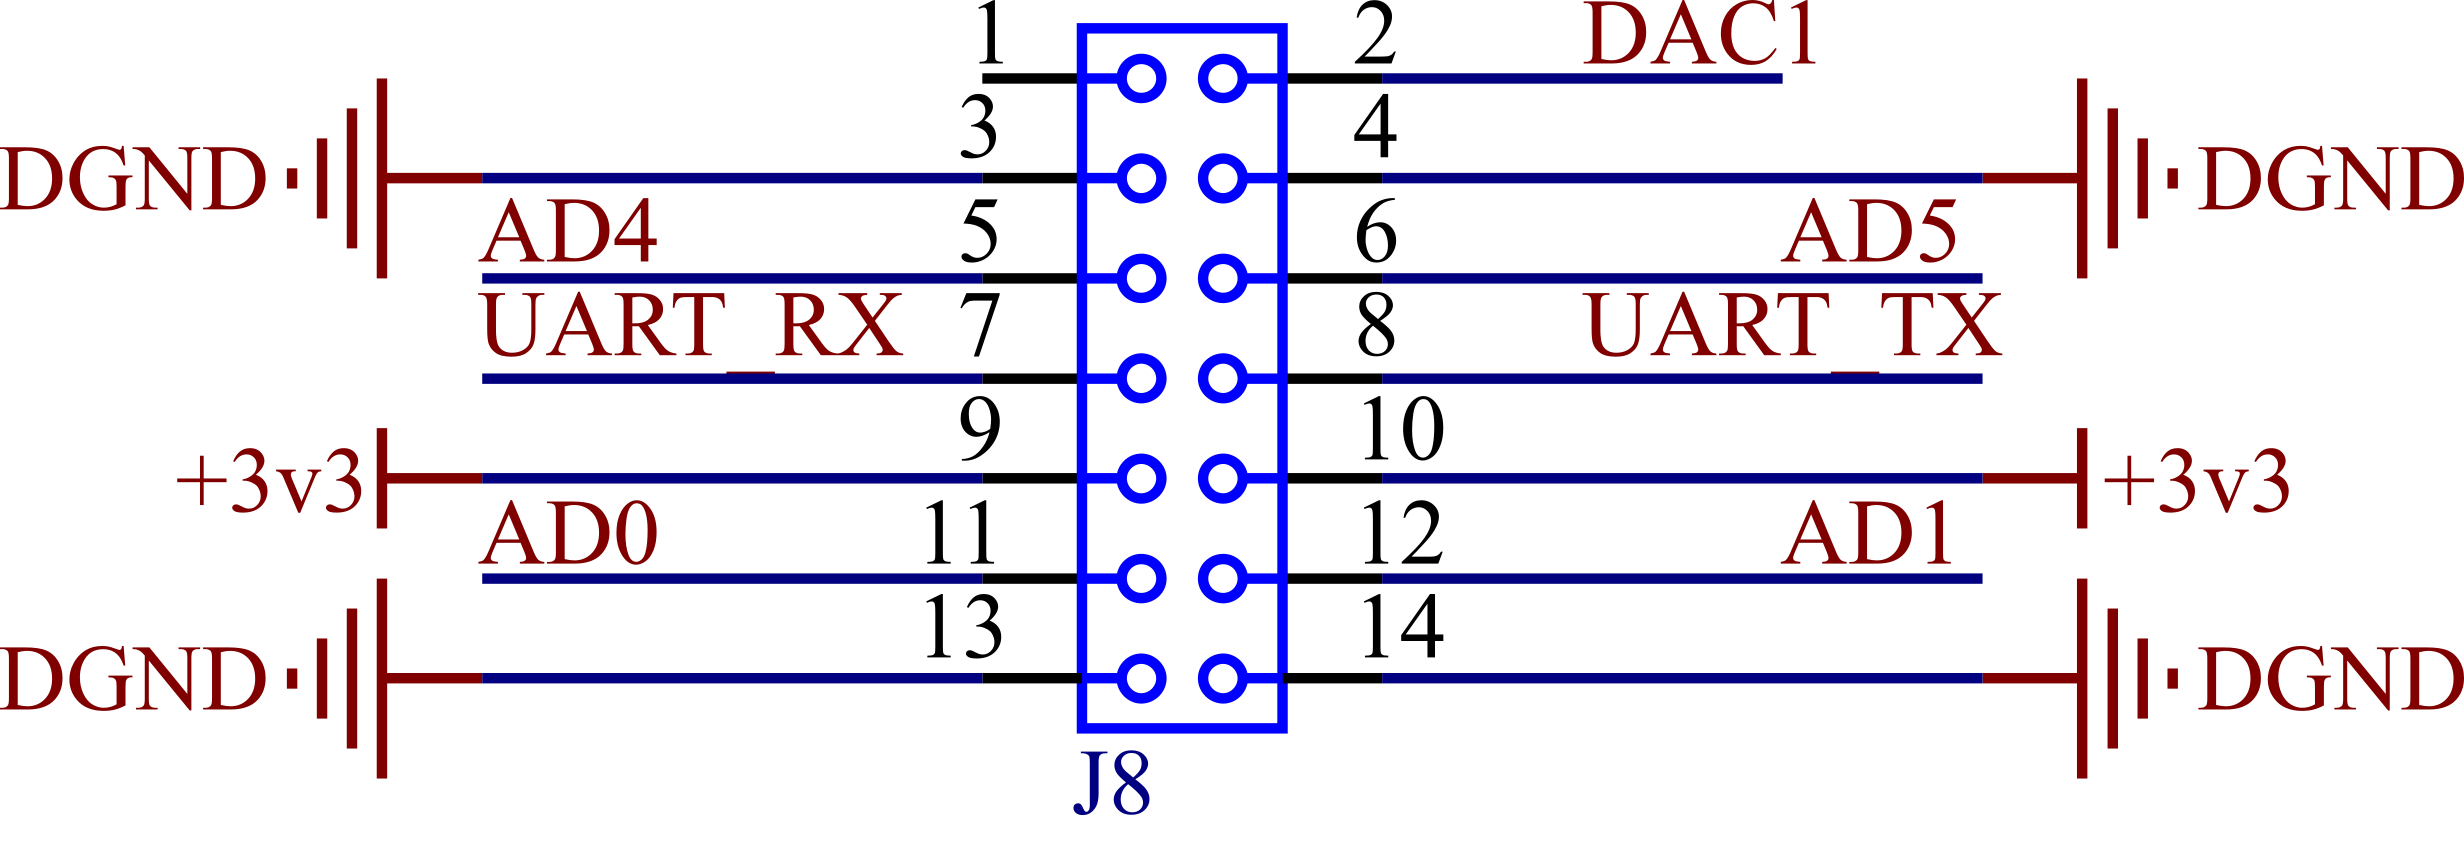
\includegraphics[scale=1.1]{../images/arm-header.png}
    \caption{Header}
    \label{fig:arm-header}
  \end{subfigure}

  \begin{subfigure}[b]{0.49\textwidth}
    \centering
    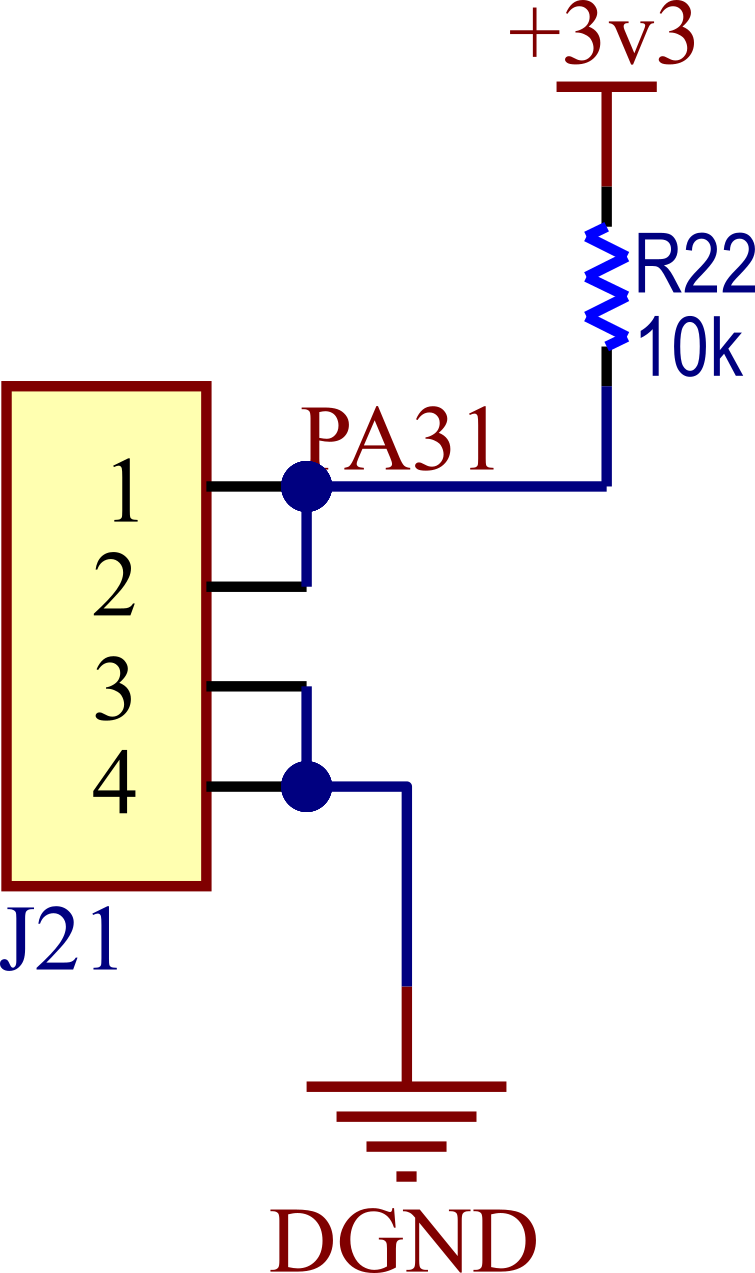
\includegraphics[scale=1.1]{../images/arm-button.png}
    \caption{Botón}
    \label{fig:arm-button}
  \end{subfigure}
  \begin{subfigure}[b]{0.49\textwidth}
    \centering
    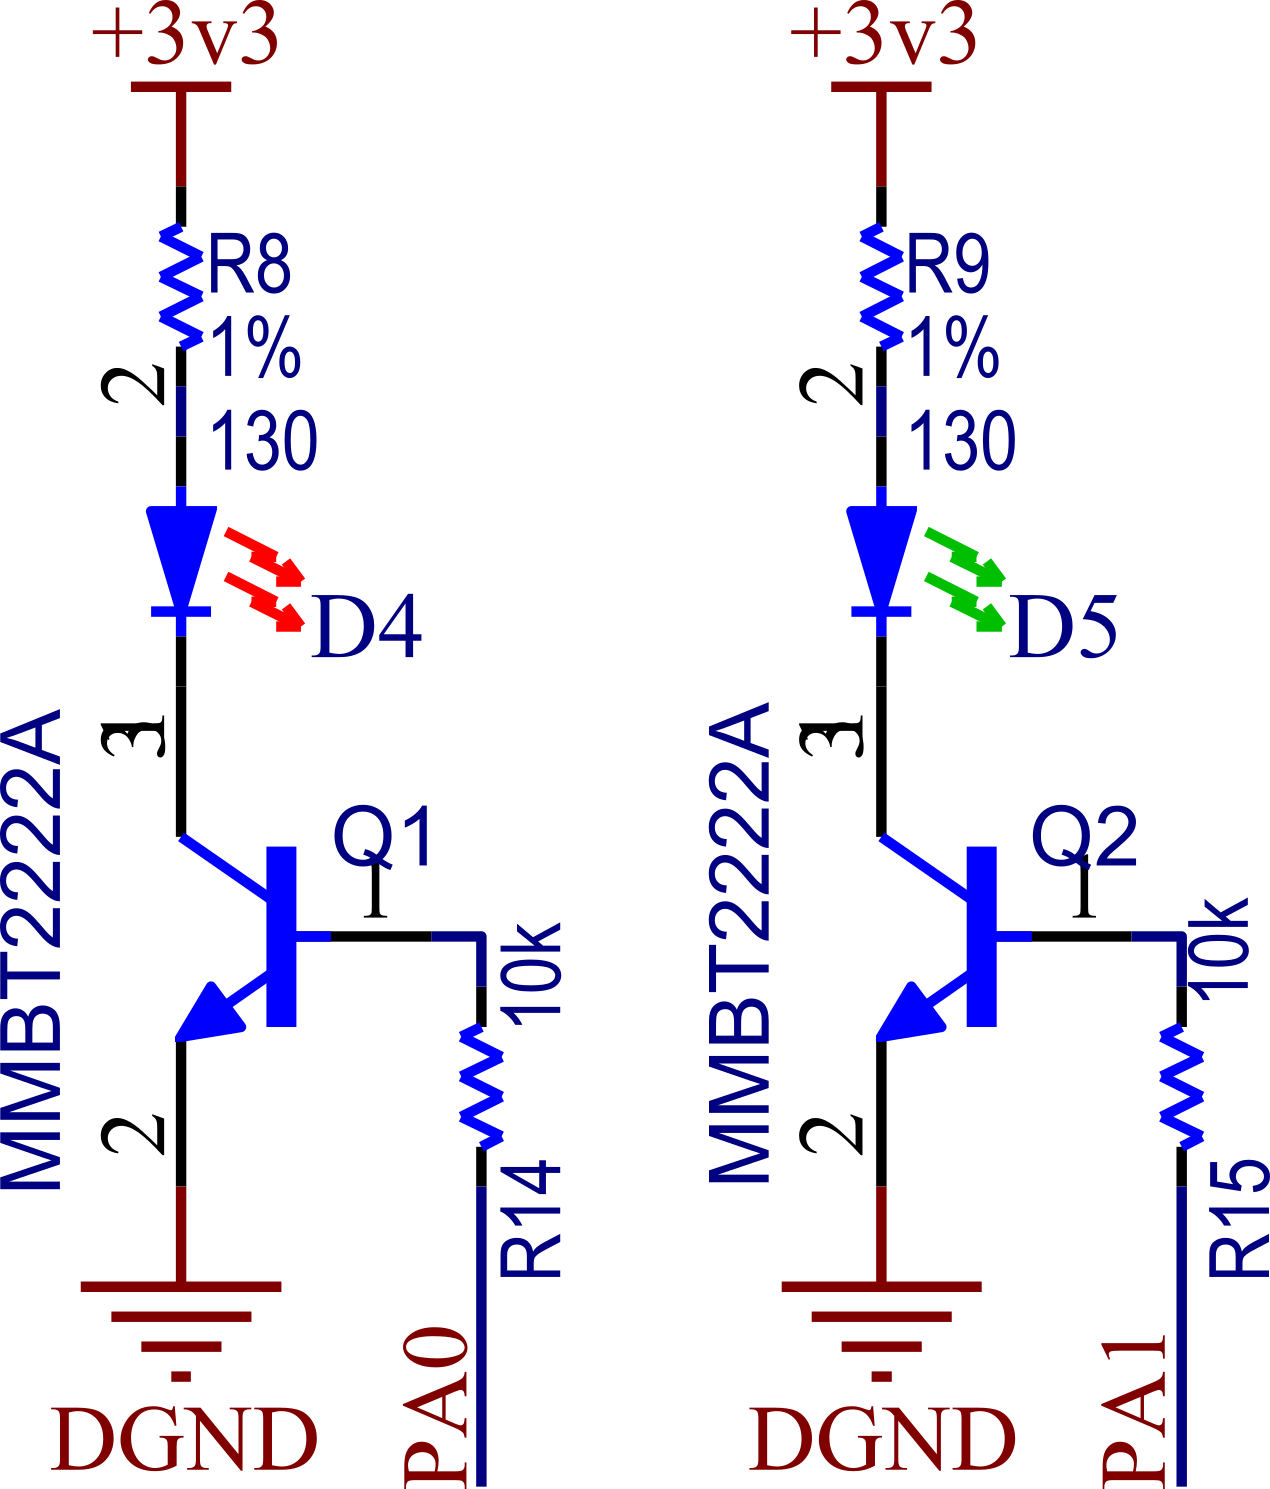
\includegraphics[scale=1.1]{../images/arm-leds.png}
    \caption{LEDs}
    \label{fig:arm-leds}
  \end{subfigure}
  \caption{Otras conexiones del microcontrolador}
\end{figure}

%% ----------------------------------------------------------------
\subsubsection{Características integrado}
%% ----------------------------------------------------------------
El microcontrolador elegido es el SAM4S8B con las siguientes características:

\begin{itemize}
  \item Frecuencia de clock \SI{120}{MHz}
  \item \SI{512}{Kbytes} de memoria Flash
  \item \SI{128}{Kbytes} de de memoria SRAM
  \item Encapsulado 64LQFP
  \item ADC 12-bit de 11 canales
  \item DAC 12-bit de 2 canales
  \item 47 puertos de entrada y salida (PIOs)
  \item 2 UART
  \item PWM, timers, I2C, SPI, y otras funciones
\end{itemize}

Se decidió utilizar la familia Atmel ya que se contaba con disponibilidad y experiencia en su uso. Este modelo en particular fue elegido por su velocidad, confiabilidad y gran capacidad de Flash y SRAM.


\end{document}